\documentclass{article}


% load package with some of the available options - you may not need this!
\usepackage[framed,autolinebreaks,useliterate]{mcode}

% for checklist
\usepackage{enumitem,amssymb}
\newlist{todolist}{itemize}{2}
\setlist[todolist]{label=$\square$}
\usepackage{pifont}
\newcommand{\cmark}{\ding{51}}%
\newcommand{\xmark}{\ding{55}}%
\newcommand{\done}{\rlap{$\square$}{\raisebox{2pt}{\large\hspace{1pt}\cmark}}%
\hspace{-2.5pt}}
\newcommand{\wontfix}{\rlap{$\square$}{\large\hspace{1pt}\xmark}}


% something NOT relevant to the usage of the package.
\usepackage{graphicx}
\usepackage{url,textcomp}
\setlength{\parindent}{0pt}
\setlength{\parskip}{18pt}
\title{ECTA Homework 3\\Shape Matching Problem}
\author{\color{blue}Arun Prabhu, \texttt{arun.prabhu@smail.inf.h-brs.de}\\
\color{blue}Dharmin Bakaraniya, \texttt{dharmin.bakaraniya@smail.inf.h-brs.de}}
% //////////////////////////////////////////////////

\begin{document}

\maketitle
\begin{center}
	\begin{minipage}{1\linewidth}
		\centering
			
\includegraphics[scale=0.6]{wingtypes.png}
	\end{minipage}
\end{center}

To optimize wings, it is useful to start with known designs and then adjust them to specific tasks. How to convert from one representation to another? In this assignment you will convert the 4-dimensional NACA wing specific representation into a general B-Spline representation with 32 control points. You will compare 2 evolutionary methods, Genetic Algorithms and Evolution Strategies.

\newpage

\section{Assignment Description}
	Shape Matching Problem
	\begin{enumerate}
		\item Write your own Genetic Algorithm to solve the shape matching problem
		\item Write your own version of the Covariance Matrix Adaptation Evolution Strategy (CMA-ES) to solve the shape problem.
		\item Compare the performance of the two algorithms on three airfoils (NACA airfoil shapes: 0012, 5522, 9735). Is there a significant difference between a GA and an ES? 
	\end{enumerate}

	\begin{itemize}
 	\item Grading Scheme
 		\begin{todolist}
 		\item Genetic Algorithm (20 pts)
 			\begin{todolist}
 			\item Bitstring \textit{or }Real-Valued ($20$ pts)
 			\item Bitstring \textit{and }Real-Valued ($+10$pts)
 			\end{todolist}
 		\item Evolution Strategies (60 pts)
 		  	\begin{todolist}
 			\item ES with $1/5$ rule ($30$ pts)
 			\item CMA-ES with out evolution paths ($30$ pts)
 			\item CMA-ES with evolution paths ($+10$)
 			\end{todolist}
 		\item Comparisons (20 pts)
 		  	\begin{todolist}
 			\item Big beautiful wall of data
 			\end{todolist}
 		\end{todolist}
	\end{itemize}
\newpage


\section{Submission Instructions}
To be perfectly clear we expect two submissions to LEA:
\begin{enumerate}
	\item 1 PDF (report) -- a modified version of your submission PDF, with your own code snippets, figures, and responses inserted
	\item 1 ZIP (code and data)   -- a .zip file containing all code use to run experiments (.m files) \textit{and} resulting data as a .mat file
	\item Make sure to follow the naming scheme\newline HW\_NUMBER\_LASTNAME1\_LASTNAME2.suffix
	\item $\rightarrow$ A valid name would be HW\_02\_Smith\_Fernandez.pdf
	\item Make sure both team members use the same filename!
\end{enumerate}

\newpage


\newpage
\section{The Assignment}

\subsection{Genetic Algorithm}
\begin{itemize}
	\item Genetic Algorithms are typically represented by a string, this string could take many forms, such as bitsrings or real-valued numbers. What are the advantages and disadvantages of each encoding in this application? How would you convert each into 32 real-valued numbers? How could you perform crossover and mutation in each? Which do you think would be best?
	\begin{enumerate}
		\item Bitstring
		\color{blue}
        \begin{itemize}
            \item \textbf{Advantages}
                \begin{itemize}
                    \item Crossover and mutation is easy perform.
                    \item Genome manipulation is faster.
                \end{itemize}
            \item \textbf{Disadvantages}
                \begin{itemize}
                    \item Difficult to represent solutions of real valued problems.
                \end{itemize}
            \item \textbf{Crossover}: One point or N point crossover.
            \item \textbf{Mutation}: A bit is flipped randomly with \texttt{mutProb} probability.
        \end{itemize}
        \color{black}
		\item Real-valued
		\color{blue}
        \begin{itemize}
            \item \textbf{Advantages}
                \begin{itemize}
                    \item Easy to represent solutions to real valued problem.
                \end{itemize}
            \item \textbf{Disadvantages}
                \begin{itemize}
                    \item Slower performance compared to bit string representation.
                    \item Difficult to perform genome manipulations.
                \end{itemize}
            \item \textbf{Crossover}: Take mean of the parents.
            \item \textbf{Mutation}: We replace a gene with a random float with \texttt{mutProb} probability.
        \end{itemize}
        \begin{lstlisting}
function num = bit2float(bitString, nBit)
[nRows, nCols] = size(bitString);
nFloat = nCols/nBit;
num = zeros(nRows, nFloat);
for r = 1:nRows
    for c = 1:nFloat
        bs = bitString(r,((c-1)*nBit+1):((c-1)*nBit+1)+nBit-1);
        number = bin2dec(num2str(bs));
        number = (number/(2^nBit)) - 0.5;                           
        num(r,c) = number;
    end
end
end
        \end{lstlisting}
        \begin{itemize}
            \item Each genome is made of \texttt{nFloat} bitstrings.
            \item Each bitstring contains \texttt{nBit} bits. 
            \item We convert it to decimal number. That decimal is divided by the range on the bitstring space($2^{nBit}$).
            \item This float value will be in range of 0 to 1. Now, we subtract 0.5 to get float values in our desired range.
        \end{itemize}
        There is no best way to solve GA problems. The representation of genome depends on the problem statement. For example, knapsack will highly benefit by the use of bitstring, but here float representation is advantageous.
        \color{black}
	\end{enumerate}
    \newpage
	\item Implement the encoding you think will perform best and plots its median performance over 20 iterations, using 20,000 evaluations.
        Figure~\ref{fig:1} \&~\ref{fig:2}
        \begin{figure}[ht!]
            \centering
            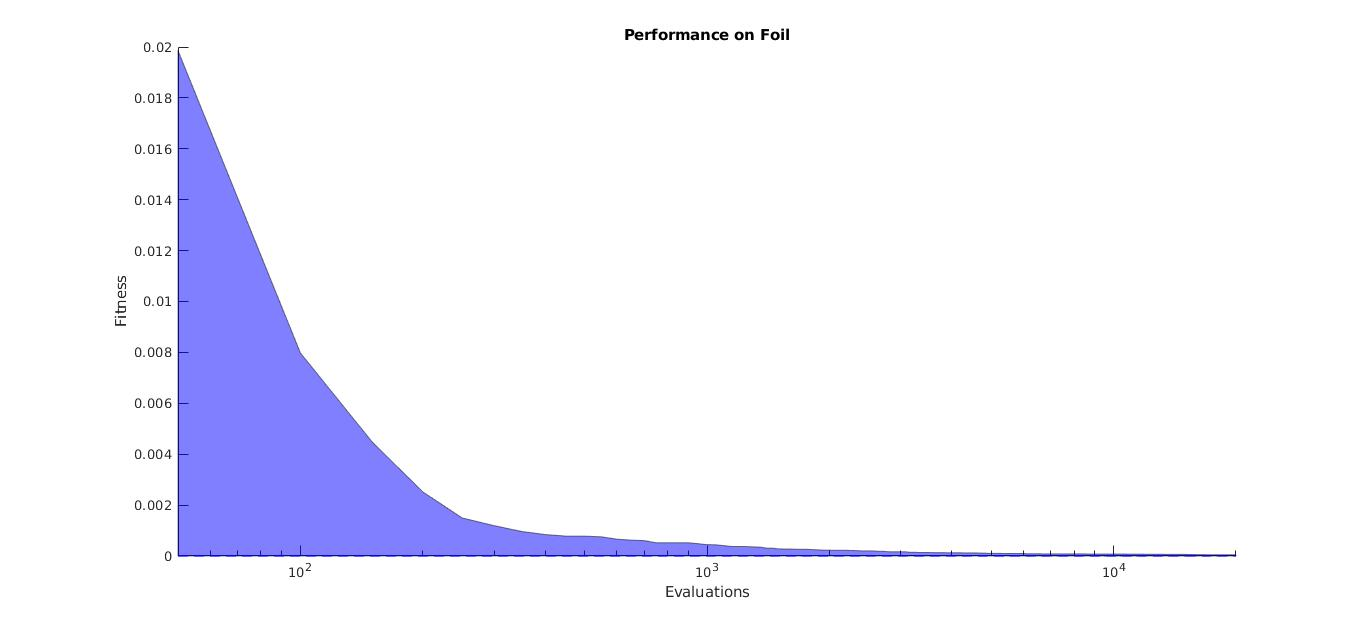
\includegraphics[width=1.0\linewidth]{ga_20exp_1foil.jpg}
            \caption{GA 20 experiments single foil (logarithmic X scale)\label{fig:1}}
        \end{figure}
        \begin{figure}[ht!]
            \centering
            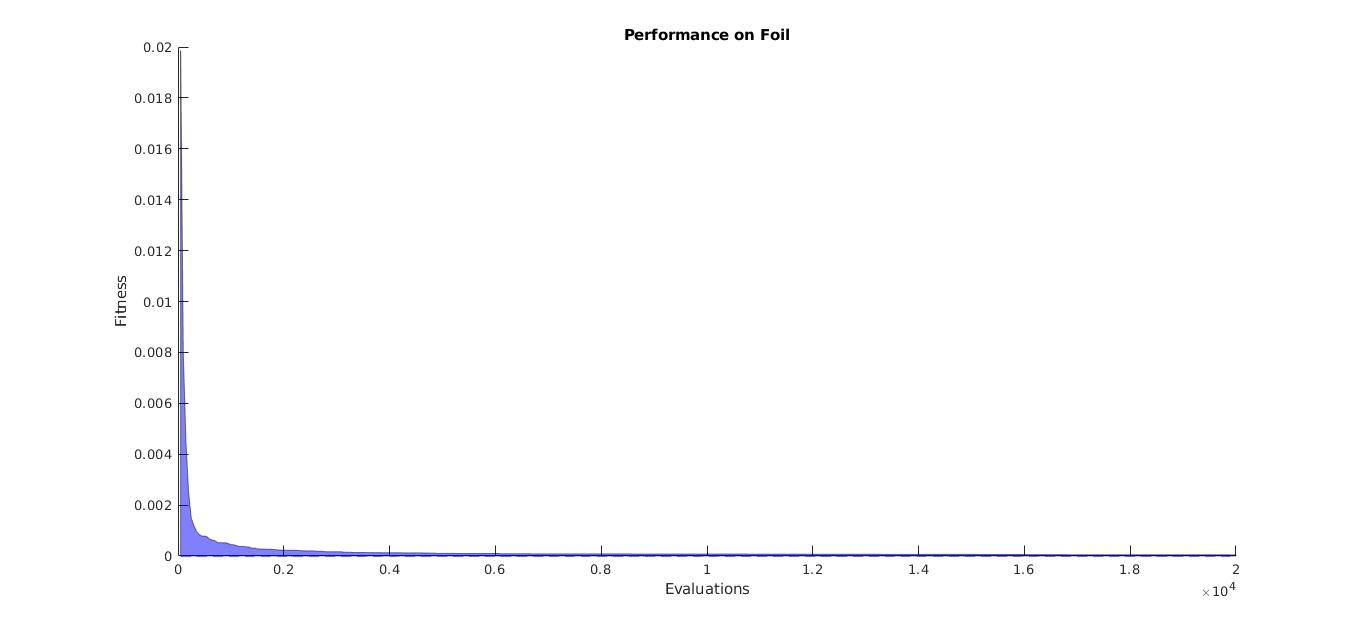
\includegraphics[width=1.0\linewidth]{ga_20exp_1foil_linear.jpg}
            \caption{GA 20 experiments single foil (Linear scale)\label{fig:2}}
        \end{figure}

        \newpage
	\item \textit{***Extra Credit***} Implement both encodings and compare them on matching task for \underline{one} of the shapes. Is one significantly better? Can you explain why?
	\color{blue}
    \begin{itemize}
        \item As seen from Figure~\ref{fig:3} and~\ref{fig:4}, GA with float genes performed better than GA with bitstring.
        \item GA with float as genes converged in less evaluations compared to GA with bitstring.
        \item The reason could be that GA with bitstring uses one point crossover which might combine unrelated genes. The conversion from bitstring to float is a slow process which made it slower.
    \end{itemize}
    \color{black}
        \begin{figure}[ht!]
            \centering
            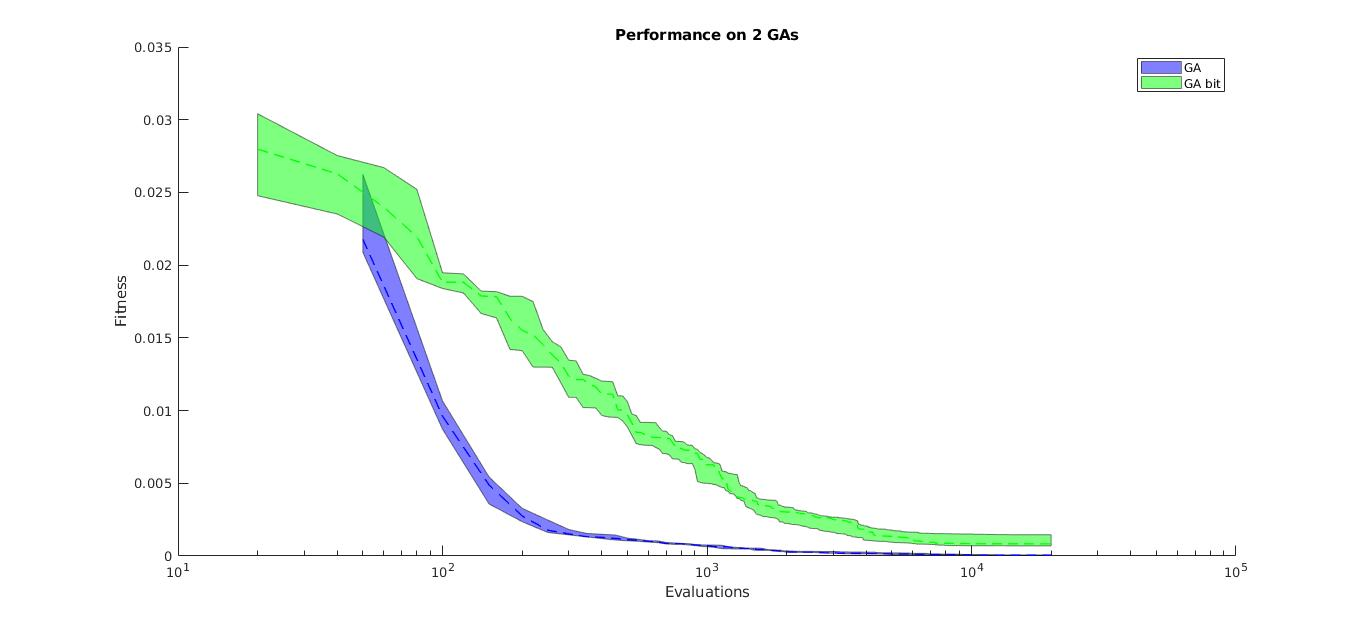
\includegraphics[width=1.0\linewidth]{ga_gaBit_20exp_3foil.jpg}
            \caption{GA vs. GA bitstring (20 experiments all foil (logarithmic X scale))\label{fig:3}}
        \end{figure}
        \begin{figure}[ht!]
            \centering
            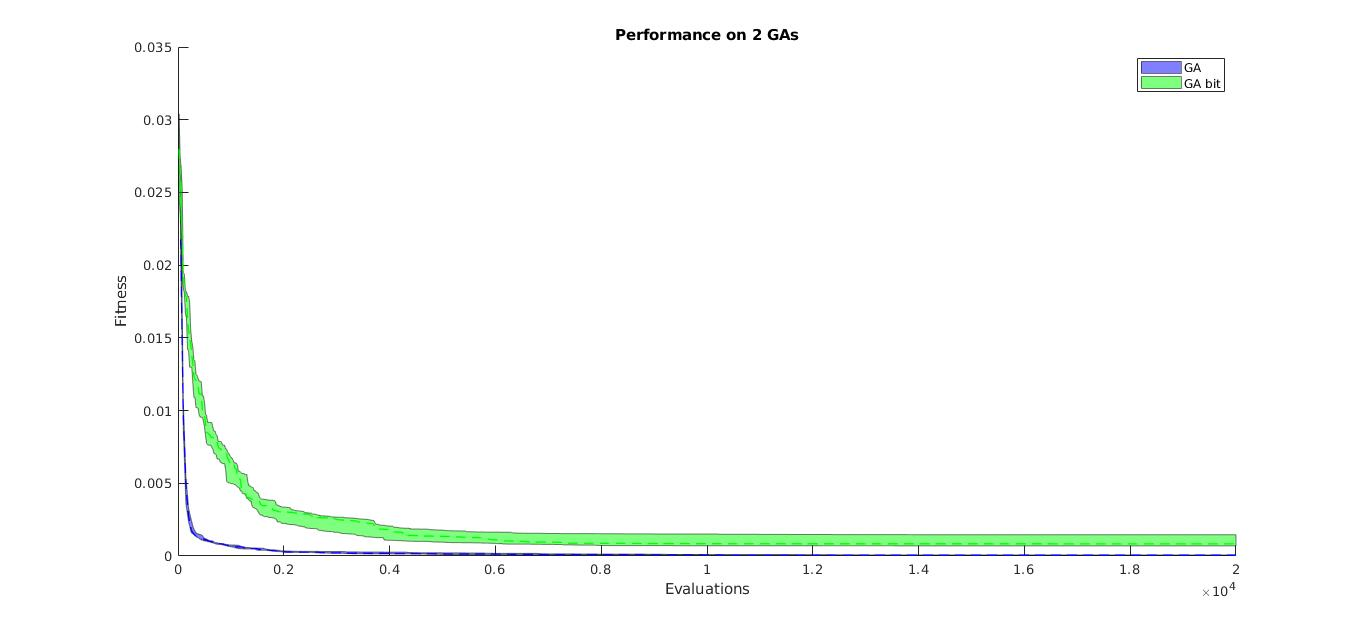
\includegraphics[width=1.0\linewidth]{ga_gaBit_20exp_3foil_linear.jpg}
            \caption{GA vs. GA bitstring (20 experiments all foil (Linear scale)) \label{fig:4}}
        \end{figure}
\end{itemize}

\newpage
\subsection{Evolution Strategies}
\begin{itemize}
	\item CMA-ES is an advanced version of ES. As a first step implement a simple ES first. 
		\begin{itemize}
			\item In this ES mutation of all parameters should have equal strength which is adjusted by the 1/5th rule.\\(\textit{every N generations change mutation strength: if $>1/5$th of mutations resulted in an better fitness (i.e. a best solution) increase mutation strength, otherwise decrease mutation strength}). Test your implementation on \underline{one} of the shapes.
			\item Compare to your best GA. Is one significantly better than the other?
			\color{blue}
            \begin{itemize}
                \item ES uses (1+1) strategy with 1/5$^{th}$ rule so it has 20000 generations while GA only has 400 generations as it has \texttt{popSize=50}.
                \item As seen in Figure~\ref{fig:5}, ES is performing significantly better.
            \end{itemize}
            \color{black}
        \begin{figure}[ht!]
            \centering
            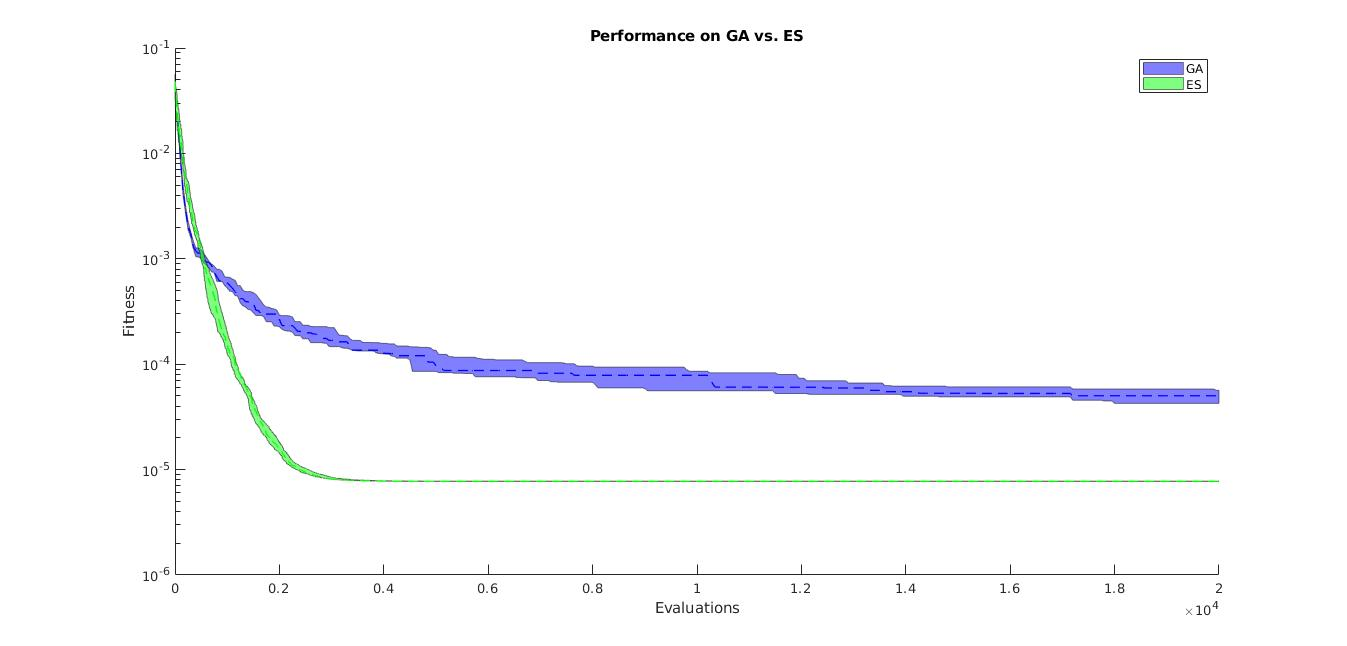
\includegraphics[width=1.0\linewidth]{ga_es_20exp_3foil.jpg}
            \caption{GA vs. ES (20 experiments all foil (logarithmic Y scale))\label{fig:5}}
        \end{figure}
		\end{itemize}
        \newpage
	\item Now program CMA-ES \underline{without evolution paths}.
	\begin{itemize}
		\item Compare to your ES results. Is a there a significant improvement?
			\color{blue}
            \begin{itemize}
                \item As seen in Figure~\ref{fig:7} and~\ref{fig:8}, ES is performing better but it is not performing significantly better. ES converges a little faster in our implementation.
                \item ES uses (1+1) strategy with 1/5$^{th}$ rule while CMA-ES has $\lambda = 10$ along with 1/5$^{th}$ rule.
            \end{itemize}
            \color{black}
        \begin{figure}[ht!]
            \centering
            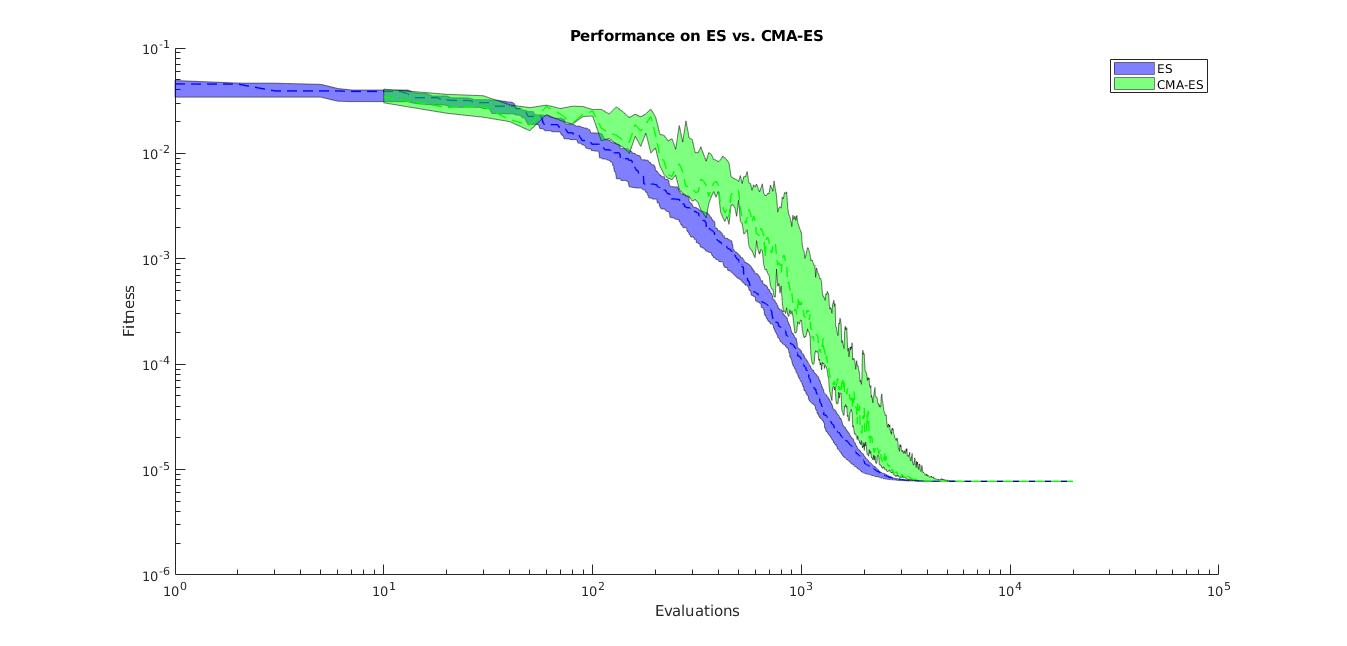
\includegraphics[width=1.0\linewidth]{es_cmaes_20exp_3foil.jpg}
            \caption{ES vs. CMA-ES (20 experiments all foil (logarithmic X \& Y scale))\label{fig:7}}
        \end{figure}
        \begin{figure}[ht!]
            \centering
            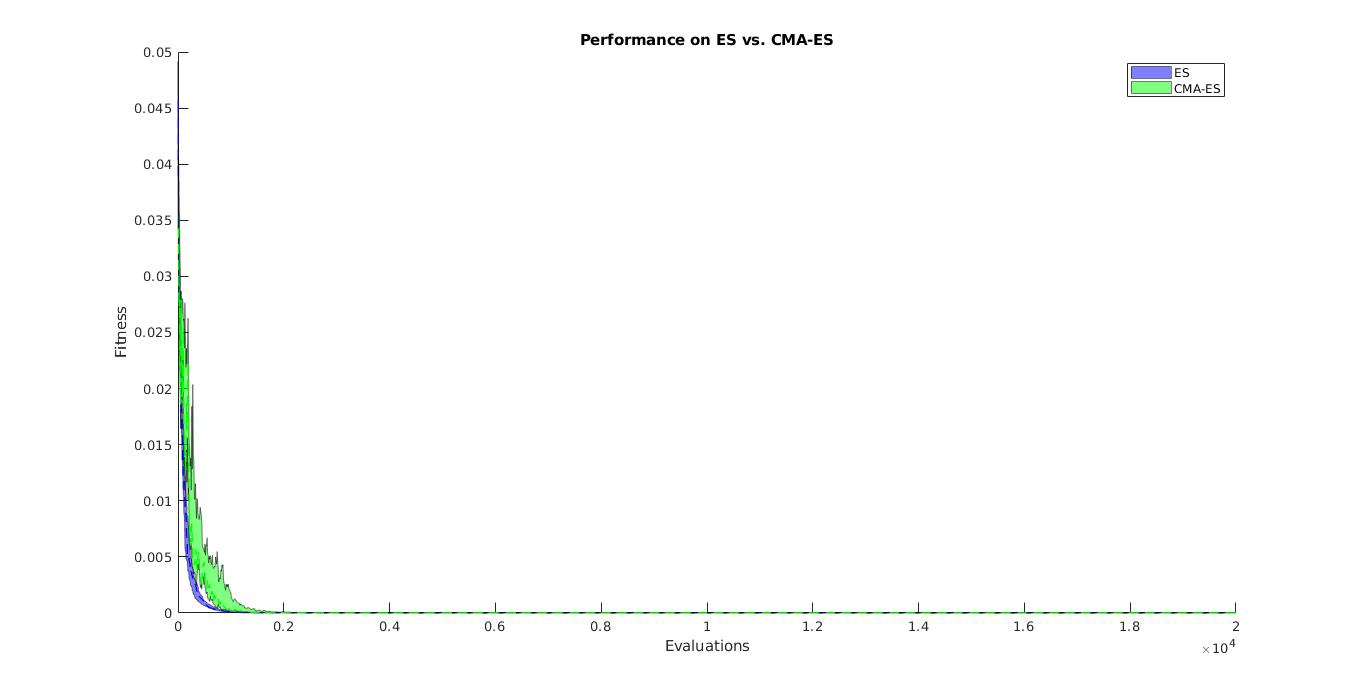
\includegraphics[width=1.0\linewidth]{es_cmaes_20exp_3foil_linear.jpg}
            \caption{ES vs. CMA-ES (20 experiments all foil (Linear scale)) \label{fig:8}}
        \end{figure}
        \newpage
	\end{itemize}

	\item \textit{***Extra Credit***} Now program CMA-ES \underline{with evolution paths}.
		\begin{itemize}
		\item Compare to your previous CMA-ES results. Is a there a significant improvement?
			\color{blue}
            \begin{itemize}
                \item As seen in Figure~\ref{fig:9} and~\ref{fig:10}, CMA-ES is performing better in our implementation.
                \item CMA-ES has $\lambda = 10$ along with 1/5$^{th}$ rule while CMA-ES EP has evolutionary path for updating covariance matrix and cummulative step length adaptation to update sigma.
            \end{itemize}
            \color{black}
        \begin{figure}[ht!]
            \centering
            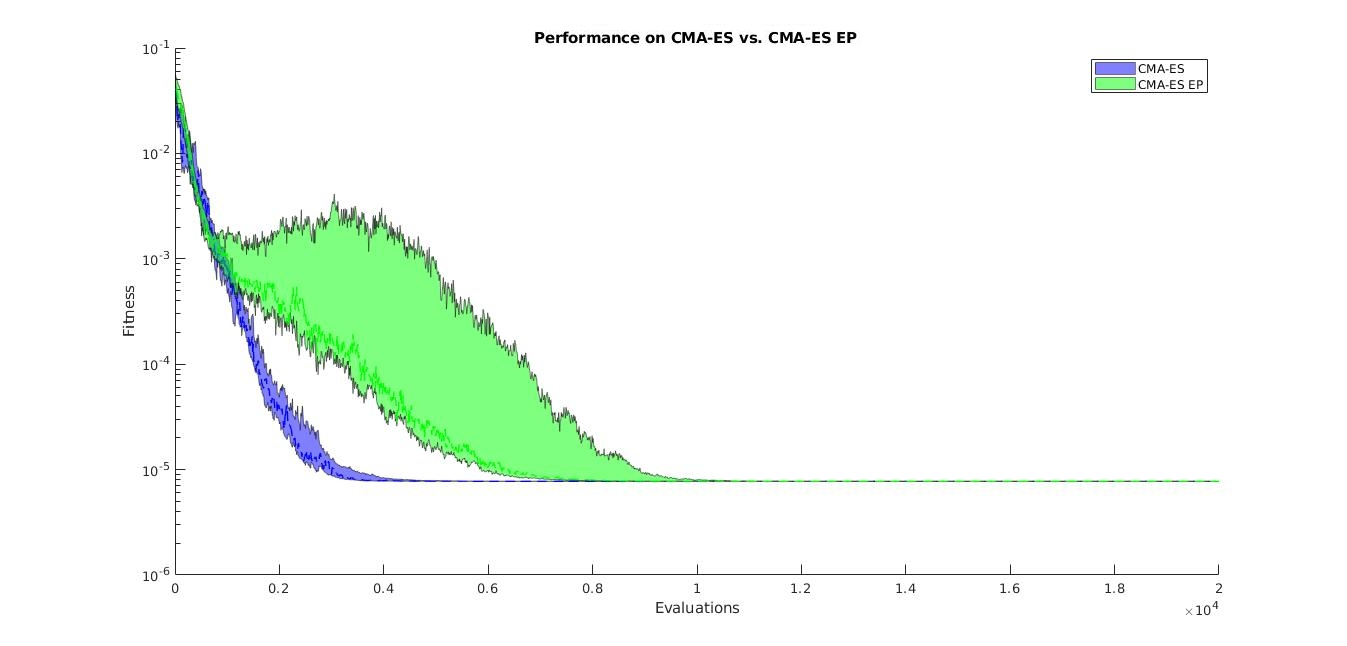
\includegraphics[width=1.0\linewidth]{cmaes_cmaesep_20exp_3foil.jpg}
            \caption{CMA-ES vs. CMA-ES EP (20 experiments all foil (logarithmic Y scale))\label{fig:9}}
        \end{figure}
        \begin{figure}[ht!]
            \centering
            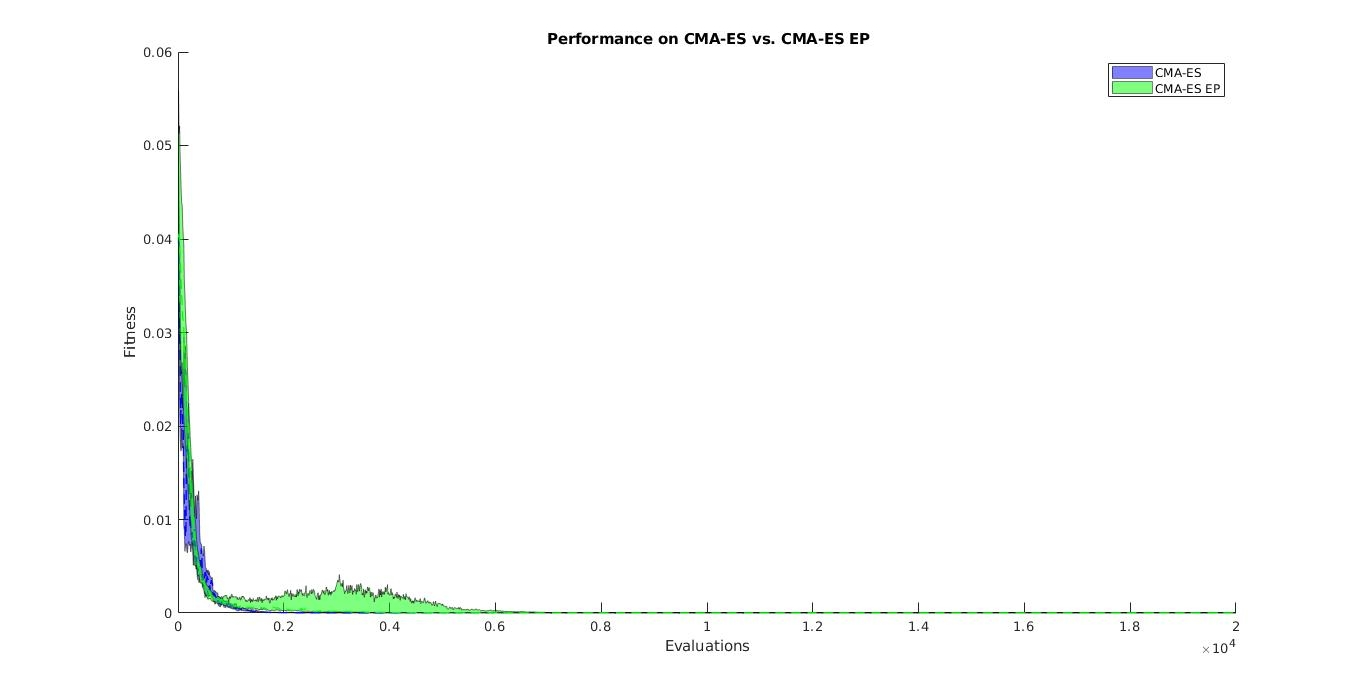
\includegraphics[width=1.0\linewidth]{cmaes_cmaesep_20exp_3foil_linear.jpg}
            \caption{CMA-ES vs. CMA-ES EP (20 experiments all foil (Linear scale)) \label{fig:10}}
        \end{figure}
		\end{itemize}
        \newpage
\end{itemize}

\newpage
\subsection{Comparisons}
Produce one plot which shows the performance of each algorithm. Run each algorthm 20 times on each shape (NACA airfoil shapes: 0012, 5522, 9735), with a budget of 20,000 function evaluations. For each run record the best ever found individual at each evaluation. For each algorithm plot the median fitness of this best ever individual. This may take some time, write a script to run and collect this data. The following should be on this plot (leaving out any algorithms you chose not to implement):
\begin{enumerate}
	\item Binary GA
	\item Real-Valued GA
	\item ES
	\item CMA-ES (without evolution paths)
	\item CMA-ES (with evolution paths)
\end{enumerate}

\color{blue}
Figure~\ref{fig:11} \&~\ref{fig:12}
\color{black}
        \begin{figure}[ht!]
            \centering
            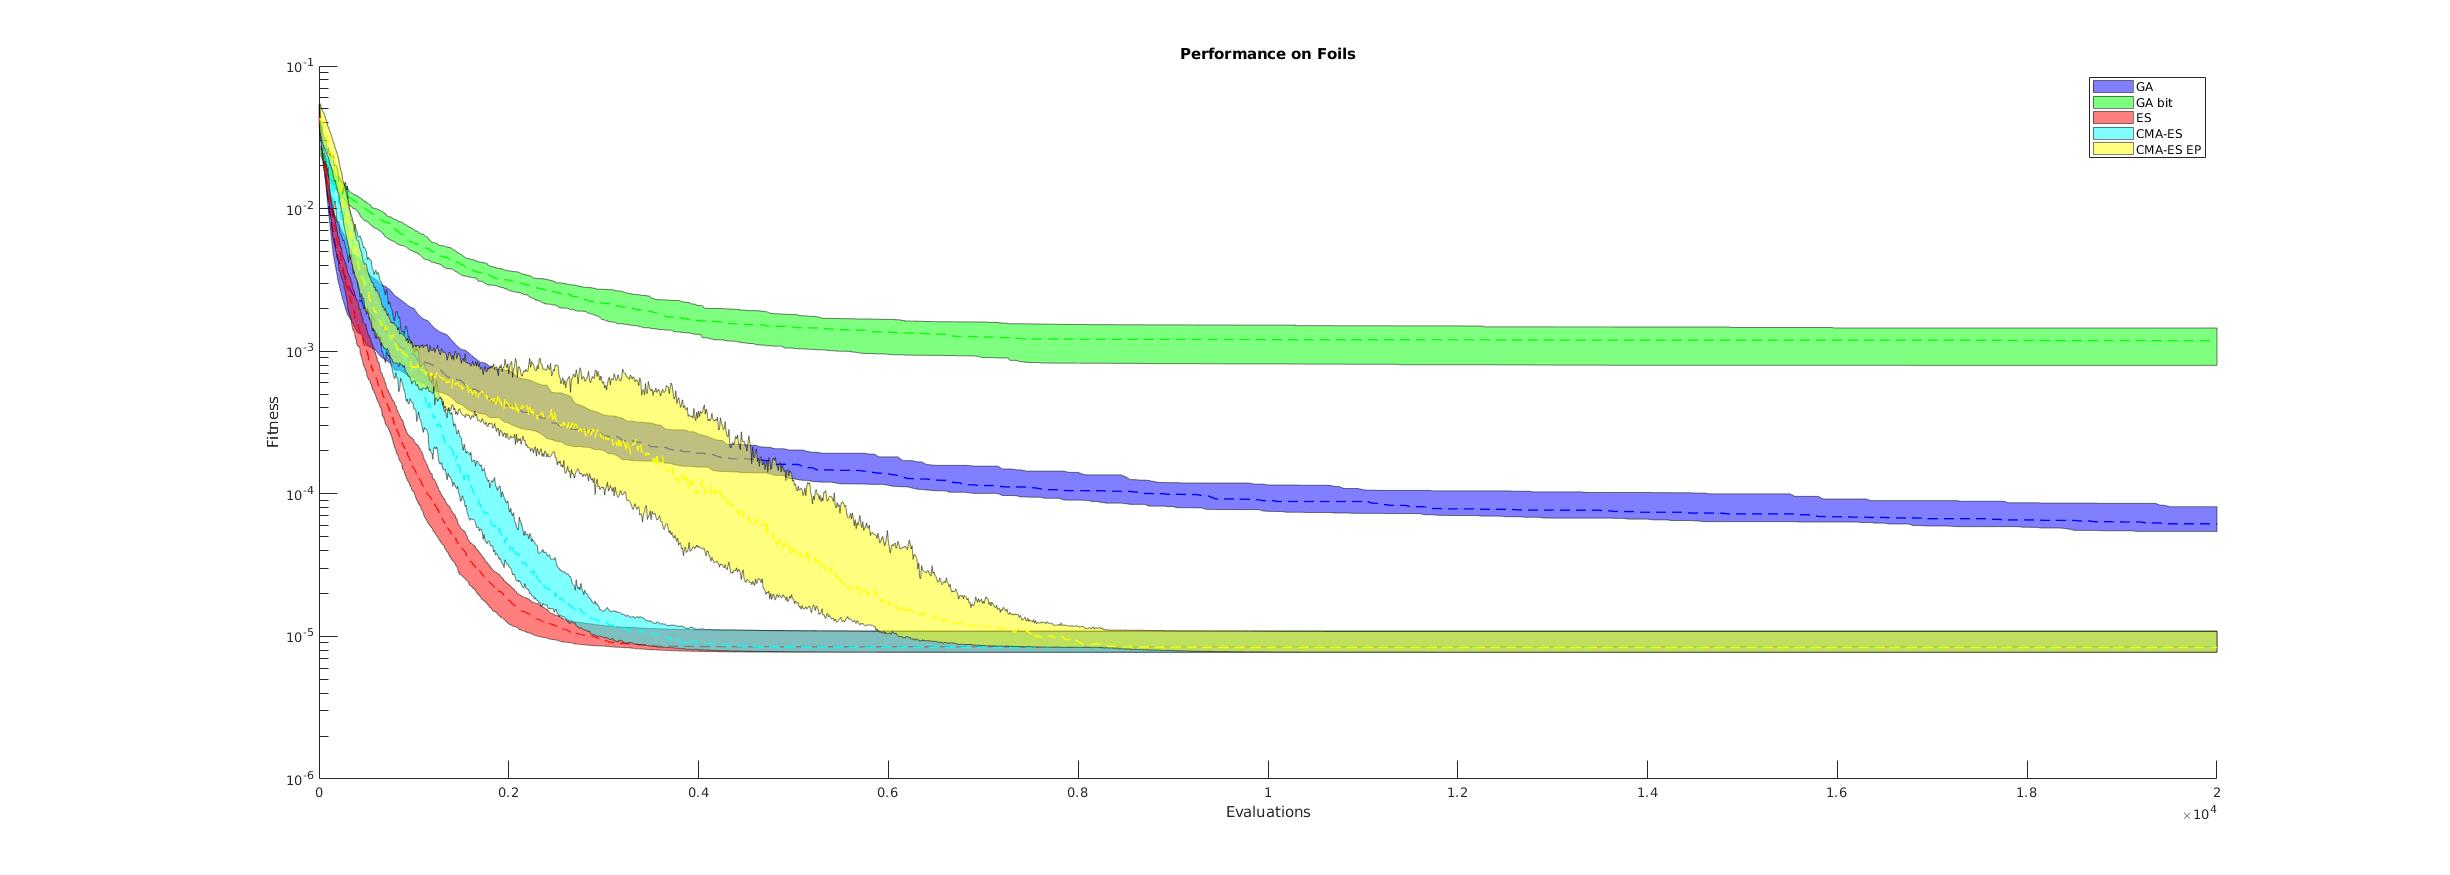
\includegraphics[width=1.0\linewidth]{output_y_log.jpg}
            \caption{All 5 algorithms (20 experiments all foil (logarithmic Y scale))\label{fig:11}}
        \end{figure}
        \begin{figure}[ht!]
            \centering
            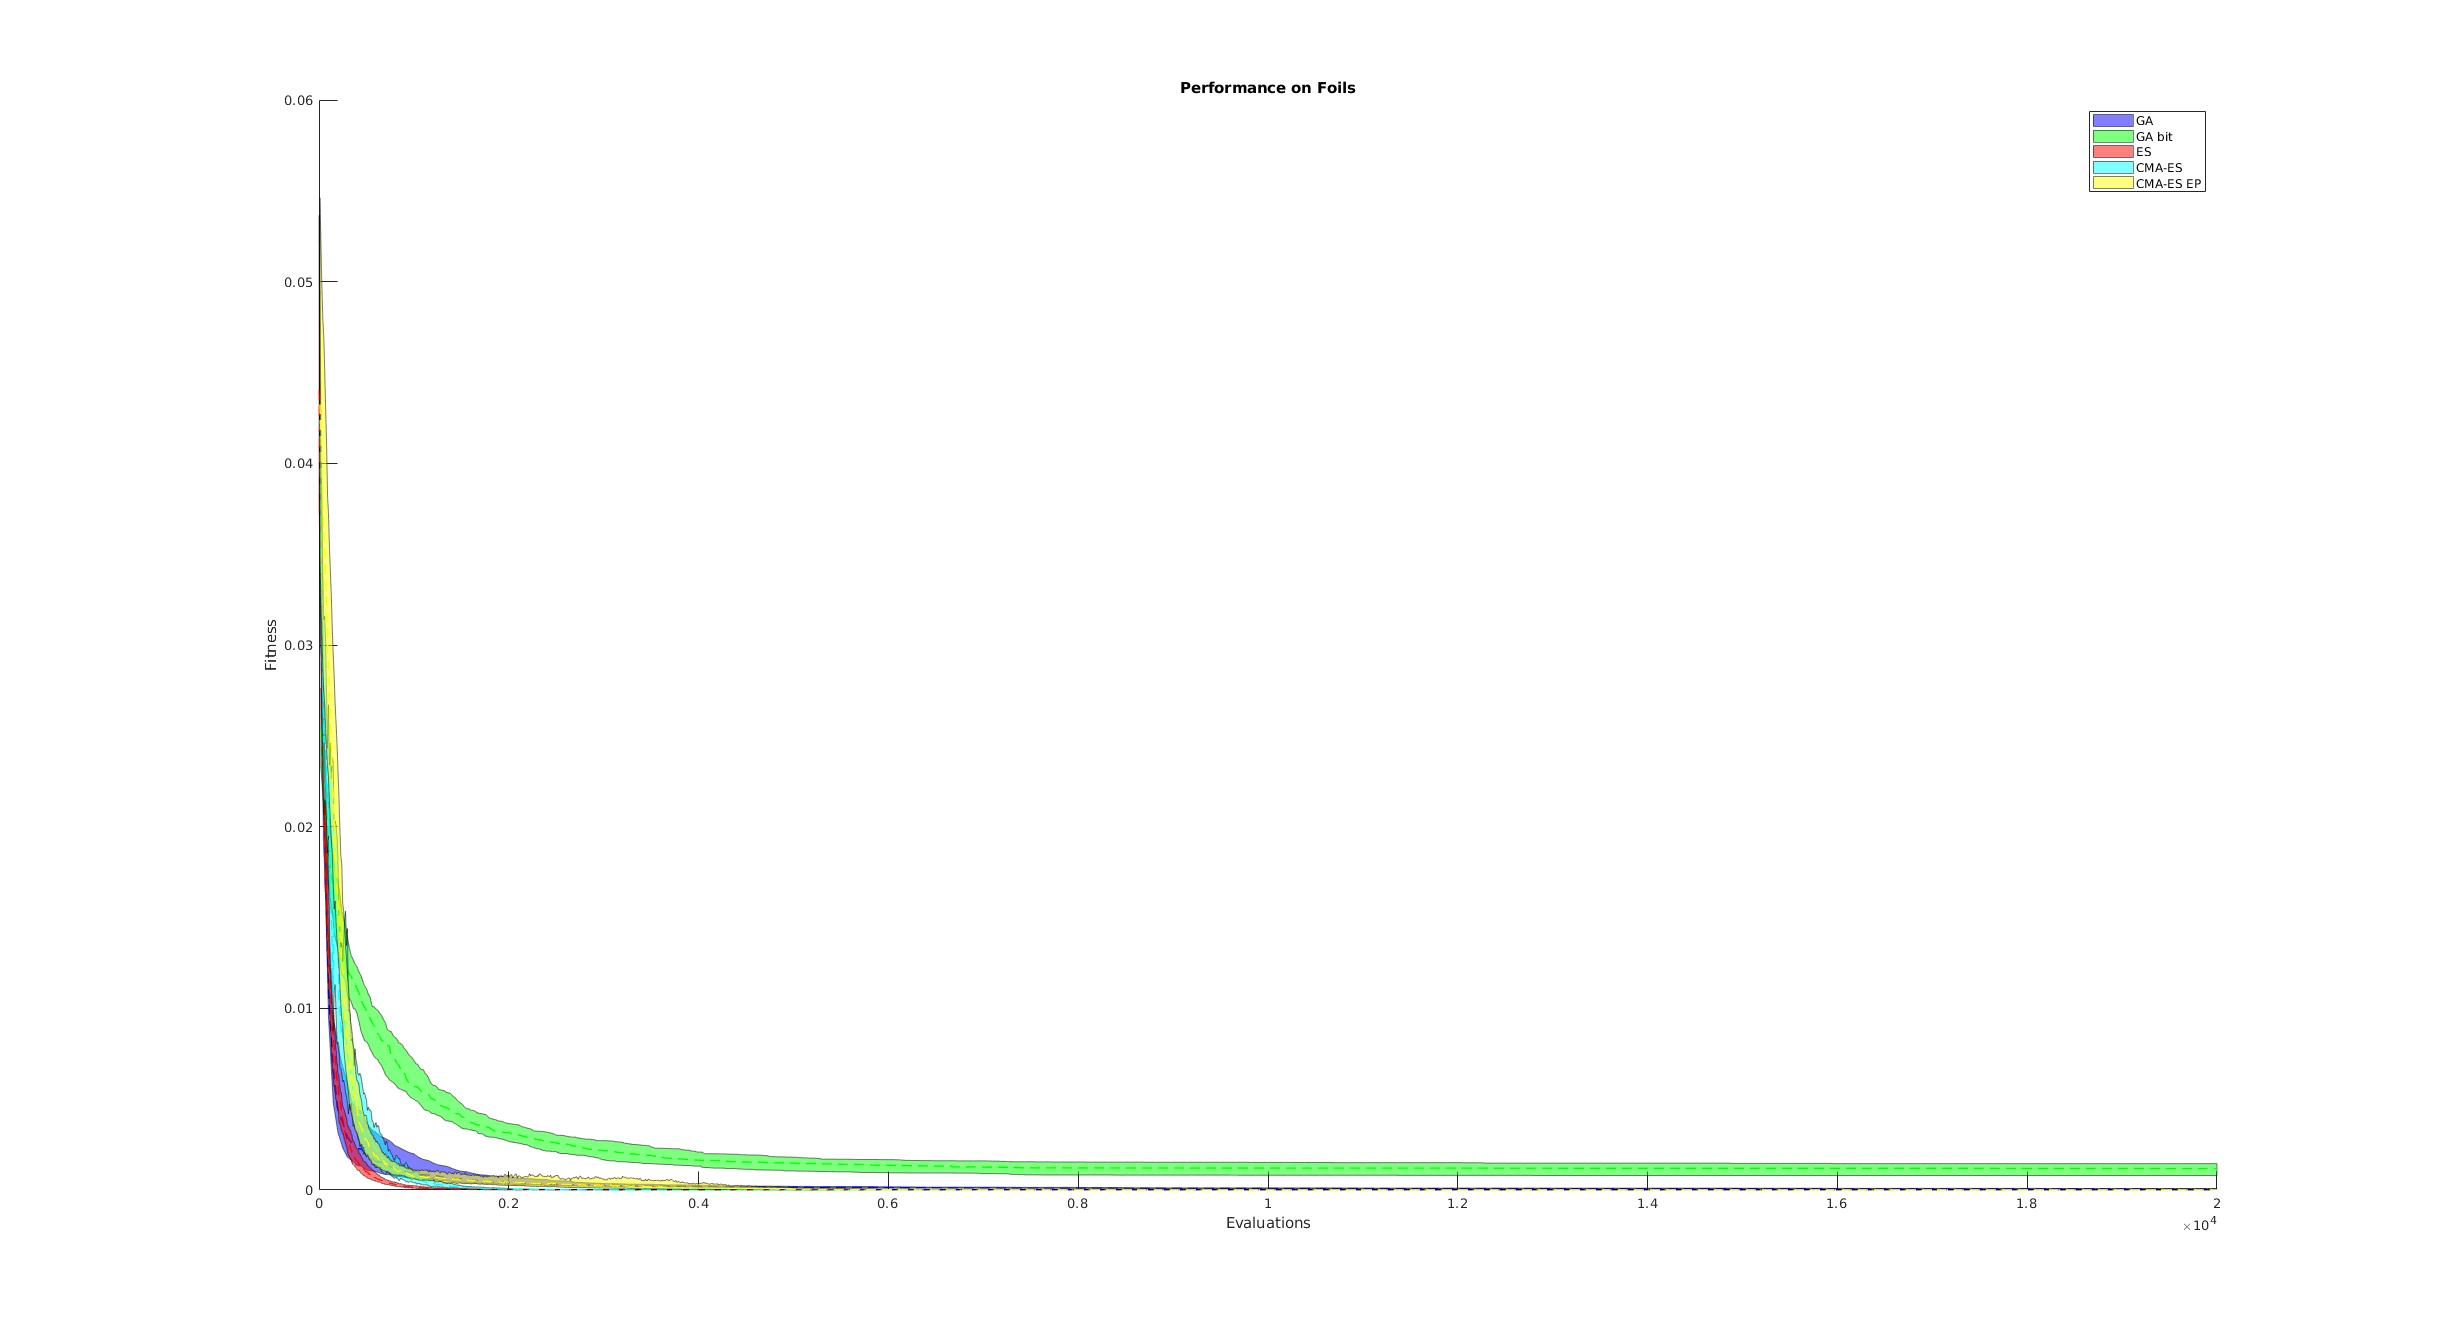
\includegraphics[width=1.0\linewidth]{outputjpeg.jpg}
            \caption{CMA-ES vs. CMA-ES EP (20 experiments all foil (Linear scale)) \label{fig:12}}
        \end{figure}





\end{document}










